\chapter{Unseen Quantum State Generation}
\label{chapter:my_contribution}
In the previous chapter we evaluated two different types of quantum GANs. The
common problem of those is the inability to generate new, unseen states. In this
chapter we propose the hybrid classical-quantum framework that can overcome this limitation. 

Our idea is based WQGANs and how the quantum Wasserstein distance is
approximated during the training. The discriminator at every step approximates
the distance between some fixed, real input state and the generated state which
changes after each iteration. However, the discriminator never needs an access to
the actual real input state, it only operates on the set of measured
expectations.

Given a parametrized circuits $U$
and set of parameters $\Theta = \{\theta_i\}$ and a set of operators $H =
\{H_j\}$, we prepare a set of vectors of expectations $S$. Each vector $s_{\theta_i}
\in S$ contains the expectations of the circuit $U(\theta_i)$, such that
$s_{\theta_i}^{(j)} = \langle H_j \rangle_{U(\theta_i)} $.

Assuming that all the vectors in $S$ come from the same distribution $p_S$,
the proposed framework is defined in two parts as follows:
\begin{enumerate}
\item \textit{Classical}: Takes as the input the set $S$ and uses it to learn a function $f:
  \mathbb{R}^{n} \to \mathbb{R}^{|H|}$. Given an arbitrary vector $z \in
  \mathbb{R}^n$ (e.g. random noise), this function produces a new vector $s' =
  f(z)$ such that $s' \sim p_S$.  
\item \textit{Quantum}: Takes $s'$ as the input and uses it as
  expectations of real input source in the WQGANs setting described in the
  previous chapter. The generator trained using $s'$ produces new, unseen before
  quantum state.
\end{enumerate}

Once the function $f$ is learnt, it can be used arbitrary many times to produce
new vectors of expectations.
With those vectors, it is possible to generate new quantum states that come from
some circuit $U(\theta')$, without ever knowing $U$ or $\theta'$.
In the following sections, we show how exactly the function $f$ can be obtained
for two different cases. 
\section{Labeled State Generation}
If the quantum state produced by the circuit $U$ can be labeled by some continuous
variable, we can use this variable to find the function $f$.

Specifically, here we assume that each parameter $\theta_i^{(j)}$ is described by some
function, i.e. $\theta_i = \theta(g_i) = [\theta^{(1)}(g_i), \theta^{(2)}(g_i), \ldots,
\theta^{(l)}(g_i)]$, for some $g_i \in V \subseteq 
\mathbb{R}$, where $l$ is the number of parameters in the circuit $U$.
We also assume that the expectations of the state produced by the
circuit $U(\theta(g_i))$, can be described by some other functions,
i.e. $s_{\theta_i} = s(g_i) = [s^{(1)}(g_i), s^{(2)}(g_i), \ldots,
s^{(|H|)}(g_i)]$, $s^{(j)}: V \to [-1; 1]\ \forall_{j \in 1,\ldots,|H|}$.
Then, the input to the classical part of the framework is the set $S$, together with
corresponding $g_i$ for each $s_{\theta_i} = s(g_i) \in S$.
To find $s^{(j)}\ \forall_{j=1,\ldots,|H|}$ functions interpolation is
sufficient. So, the function $f: V \to \mathbb{R}^{|H|}$ simply takes
any value of $g \in V$ and returns the expectations for this value using
interpolations of functions $s^{(j)}$.

This approach can be used when $U$ is the topological phase transition circuit from
Appendix \ref{apx:topological_phase_transition_ansatz}. All the parameters of
this circuit can be described by three functions $\theta_v, \theta_w, \theta_r$
for $g \in V = [1; -1]$. To prepare the input to the classical part 
 $m$ values of $g$ are sampled and the expectations of $U(\theta_v(g_i),
\theta_w(g_i), \theta_r(g_i))\ \forall_{i=1,\ldots,m}$ for all k-length Pauli
Strings operators are calculated. This data is used to interpolate the expectation functions for those
operators.  
In Figure \ref{fig:phase_exps} interpolated expectations of the circuit for
$k=3$ and $m=11$ are plotted (only subset of the expectation is plotted for readability).

\begin{figure}[htbp!]
  \captionsetup[subfigure]{labelformat=empty}
  \centering
  \subfloat{
    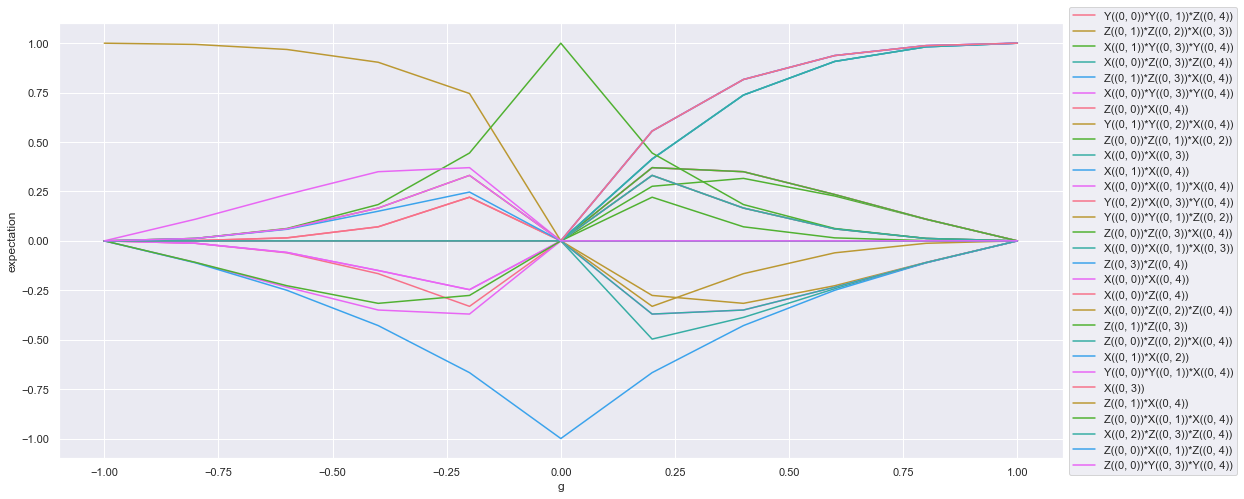
\includegraphics[width=1\linewidth]{figures/phase_exps/plot.png}
  }
  \label{fig:phase_exps}
  \caption{Interpolated expectations of topological phase transition circuit (Appendix
    \ref{apx:topological_phase_transition_ansatz}) with 5 qubits width for 20
    random 3-Pauli Strings operators. Interpolation using evenly
    spaced 11 values of the parameter $g \in [-1; 0]$. 
  }
\end{figure}

The interpolated expectations are used to learn the quantum states for
the values of $g$ that were not part of the classical part input. [PLOT]

\section{Unlabeled State Generation}
text

%%% Local Variables:
%%% mode: latex
%%% TeX-master: "../main"
%%% End: